\documentclass{article}
\usepackage{natbib}
\usepackage{wrapfig}
\title{Exercises on instrumental variables (IV) concepts and methods }
\date{ICPSR Session 2 (July 19, 2021)}


\usepackage{icpsr-classwork}

\begin{document}
\maketitle

\begin{minipage}{1.0\linewidth}

\begin{wrapfigure}{r}{.65\linewidth}
\igrphx{albertsonLawrence2009tab1}
\end{wrapfigure}

The table at right comes from Albertson and Lawrence's (2009, \textit{Amer. Pol. Res.} \textbf{37}/2) paper ``After the credits roll: The long term effects of educational television on public knowledge and attitudes,'' which reported on two field experiments. (You'll find a PDF in \texttt{articles/applications/}.)   Besides being thematically related, the two experiments followed very similar designs, using random digit dialing (RDD) telephone sampling to recruit initial samples, then employing a randomized encouragement design.  Common methods estimate the CACE (LATE) under the following assumptions:

\begin{itemize}
\item Random assignment: $\mathrm{Pr}(Z_{i}=1) = $ constant over study population;  and $\mathrm{Z} $ is determined by coin tosses, card shuffles or equivalent methods
\item Excludability (for all $z$, $d$, $y_{Z=z, D=z} \equiv y_{D=d}$)
\item $p_{c} = \mathrm{Pr}(\mathrm{Complier}) > 0$ 
\item No interference 
\item Monotonicity (no defiers) 
\end{itemize}
  
\end{minipage}
\vspace{4ex}

\begin{enumerate}
\item \label{item:1}Assuming (for this question) that the IV assumptions are valid as applied to the Round 2 respondents of each experiment, estimate the ACE of encouragement to view the program on program viewing. (If you're working with a partner, divide the two experiments between you, and explain your answers to one another when you're done.)
\item Describe a hypothetical outcome variable that you would have collected, for the/one of the experiments you answered~(\ref{item:1}) about,  had you written the study questionnaire. Posit a hypothetical value for your estimated ACE of encouragement on this outcome; combine this and your answer to (\ref{item:1}) to furnish a (hypothetical) Bloom-type estimate of the complier average causal effect (CACE).  
\item Response rates for the Round 1 RDD sample recruitment effort are not reported in the table. Would you need to know these response rates in order to evaluate the IV assumptions as applied to a ``study population'' of Round 1 respondents?  As applied to a study population of Round 2 respondents? 
\item Would you need to know the Round 1 response rates in order to evaluate the generalizability of each experiments's findings to the populations described in ``Location of broadcast''?  Would they be relevant?  
\item Whether a subject responds at round 2, $R$, can be considered as a (secondary) outcome. Let $r_{Ti}$ be an indicator of whether subject $i$ would respond at round 2 if assigned to the encouragement condition, with $r_{Ci}$ denoting $i$'s corresponding potential response if assigned to control.
  \begin{enumerate}
  \item Explain why the Random Assignment assumption would be violated for a study population consisting of \textit{Round 2} respondents, despite proper use of random assignment procedures during Round 1, if it's common that $r_{T}=1$ while $r_{C}=0$.
  \item Conversely, explain how for a study population of Round 2 respondents, Random Assignment follows from a combination of Random Assignment at round 1 plus an additional assumption that $r_{Ti} \equiv r_{Ci}$, all $i$. 
  % \item What pieces of information that are necessary to appraise the plausibility of Albertson and Lawrence's (2009) random assignment assumption are missing from the table? 
  \end{enumerate}

\end{enumerate}



\begin{tabular}{c}
  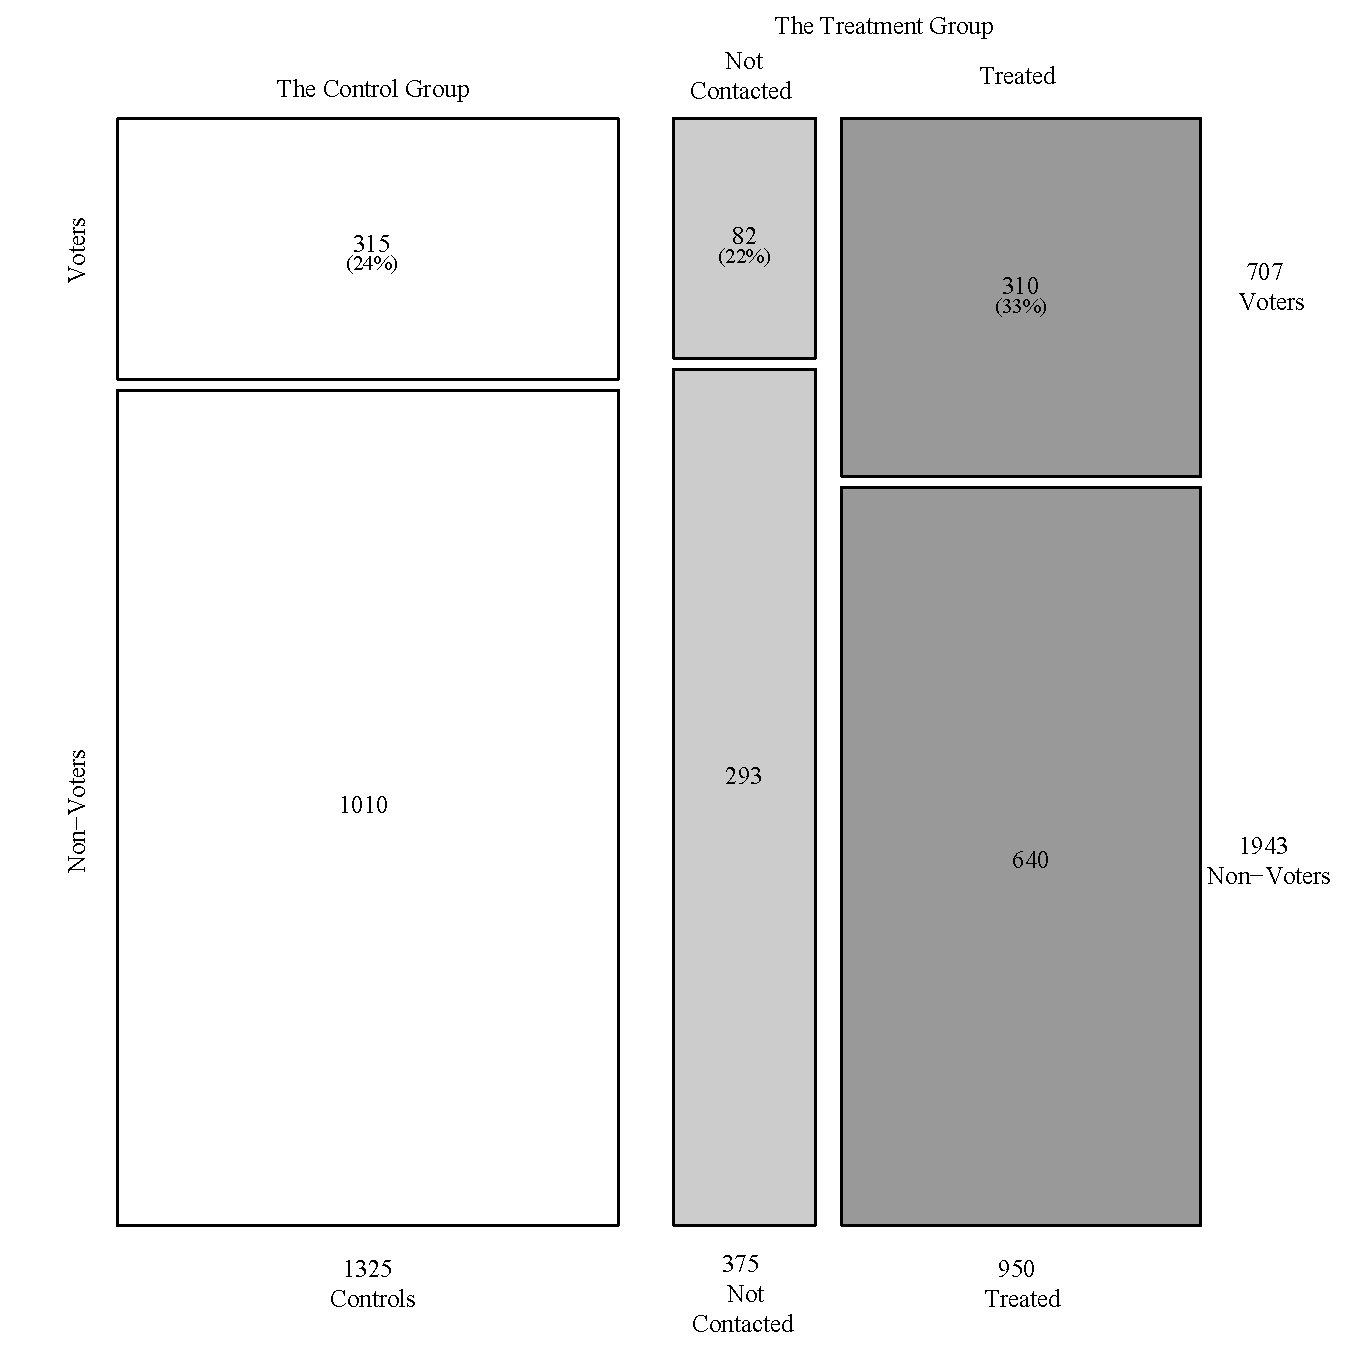
\includegraphics[height=.5\textheight]{images/ASdesign2edited}  \\
\igrphx{SalkVtable-full}
\end{tabular}

\end{document}
